% File generated by nTex - Java Application for fast notes in LaTeX
% by Jarda Vitku

\documentclass[journal,onecolumn]{IEEEtrancz}
% zvolte kodovani
\usepackage[utf8]{inputenc} % linux/unix
%\usepackage[latin2]{inputenc}
%\usepackage[cp1250]{inputenc} % Windows
\usepackage[czech]{babel}
\usepackage{graphicx}
\usepackage{makeidx}         % allows index generation
\usepackage[bookmarks=false, colorlinks=false, unicode]{hyperref}

%\usepackage{enumitem}
%\setlistdepth{9}

\begin{document}

\title{Poznámky z knihy Evolving Brains}
\author{Jaroslav Vítků}

\maketitle

\begin{abstract}
Poznámky slouží jako podklad ke zkoušce z předmětu Evoluce Nerového Systému na Univerzitě Karlově. Josu to vypsané poznámky z knihy Johna Allmana \cite{kniha}. Další poznámky (z přednášek) jsou umístěny ve složce pro předmět, jak v textové podobě, tak z pozdějších přednášk přímo ve slidech. Tento text je tříděn hlavně podle kapitol v knize. 
\end{abstract}

\IEEEpeerreviewmaketitle



\section{Brain Basics}


\begin{itemize}
	\item nejjednodussi organismus ktery projevuje znamky:
	\begin{itemize}
		\item uceni
		\item pameti
		\item rozhodovani
		\item kontrola toku informaci
			\vspace{3mm}
	\end{itemize}
	je E.coli, jednobunecna bakterie pritomna treba ve strevech
		\item 
\begin{itemize}
		\begin{itemize}
			\item umi pouze 2 pohyby (dopredu, prekulit se), ale integruje data z vice nez 12ti senzoru
				\vspace{3mm}
		\end{itemize}

	\end{itemize}

	\item nervous systems are like hybrid computers that utilize both analog and digital signals and this gain advantages offered by both modes of computation ....
		\vspace{3mm}
	\item komunikace pomoci akcnich potencialu je pritomna v jellyfish - meduze
\end{itemize}
 	-meduzy jsou nejjednodussi zvirata s nervovou soustavou


\begin{itemize}
	\item uplne puvodni pradyby prisly na to ze si muzou obalit axony tukem - myelinem
	\begin{itemize}
		\item to hodne prispelo k rozvoji vetsich mozku - lepsi prenos signalu - dal
			\vspace{3mm}
	\end{itemize}

	\item animals with large brains are rare
	\begin{itemize}
		\item there are big costs for brains
		\item brain must compete with other body organs for the limited amount of energy available
		\item this is powerful constraint on the evolution of large brains
			\vspace{3mm}
		\item large brains demand also long time to mature
		\begin{itemize}
			\item this decreases the rate with which can be animals reproduced
			\item and it requires living in a groups - communication...
		
		
\end{itemize}
	\end{itemize}
\end{itemize}
\section{Comparing Brains}


nejjednodussi moznost:
\begin{itemize}
	\item 
	\begin{itemize}
		\item porovnvat absolutni vahu 
		\begin{itemize}
			\item neumime vsak dobre urcit co k cemu v mozku je, proto je to nepresne
		\end{itemize}

		\item provnavat na jedne ose vahu mozku, na druhe ose vahu zvirete
		\begin{itemize}
			\item na ose Y vaha mozku, na ose X vaha zvirete, cim vic vlevo nahore, tim lip
			\item diky tomu dostaneme typy mozku do jednoznacnych polygonu
				\vspace{3mm}
			\item nejvetsi mozky (stejne tak jako neocortex) maji savci
			\item obecne vetsi mozky teplokrevna zvirata (potrebuji se umet o sebe postarat-udrze teplotu)
			\item nejvetsi mozky z ryb maji zraloci a rejnoci, takze velikost mozku je casto spjata s dravosti 
			\begin{itemize}
				\item zvire bud v klidku zere listi a je hluopy, nebo vymejsli jak lip ulovit zvire a je chytry
			\end{itemize}

			\item pak jsou taky relativne chytry ptaci (ale maj jinak postavenej mozek)
			\item nejvetsi rozdily mezi rybami jsou mezi kostnatymy rybami, je to tim ze je jich 25 000 druhu
			\begin{itemize}
				\item prikladem je elephant-nosed fish Obr.\ref{elephant}, ktera se orientuje pomoci elektrickych signalu - velky mozek

				\begin{figure}[ht]
					\centering
						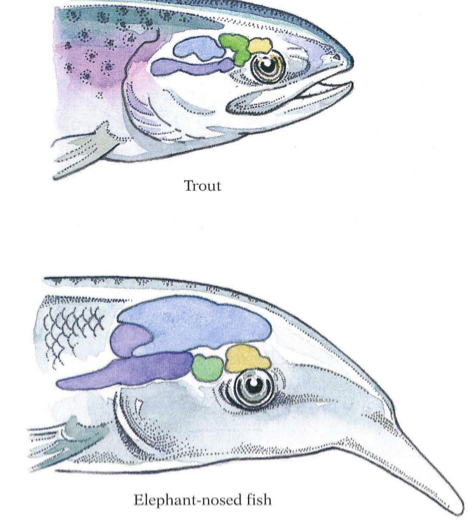
\includegraphics[width=5.0cm]{fig/elephant.png}
					\caption{Elephant nosed fish  orientuje se pomoci elektrickych signalu prot ma vyvinutou specifickou oblast mozku - jina struktura}
					\label{elephant}
				\end{figure}

					\vspace{3mm}
					\vspace{3mm}
			\end{itemize}
		\end{itemize}
	\end{itemize}
\end{itemize}
serotonin:
\begin{itemize}
	\item 
	\begin{itemize}
		\item dulezity pro evoluci mozku
		\item serotogenicky system 500 milion let stary - zachovan v evoluci porat
			\vspace{3mm}
		\item axony techto neuronu uvolnuji serotonin
		\item v mozku jich je jenim asi 100 000 (miliontina z celku)
		\item jsou ale huste propojeny vsude kolem a tak i presto ovlivnuji funkci prakticky kaudeho neuronu v mozku
			\vspace{3mm}
		\item serotonin ovlivnuje krevni tlak, zazivani a tak
			\vspace{3mm}
	\end{itemize}
\end{itemize}
mutace DNA:
\begin{itemize}
	\item 
	\begin{itemize}
		\item jsou zmeny specifickych aminokyselin na danych pozicich v DNA sekvenci Obr.\ref{chrom} 

		\begin{figure}[ht]
			\centering
				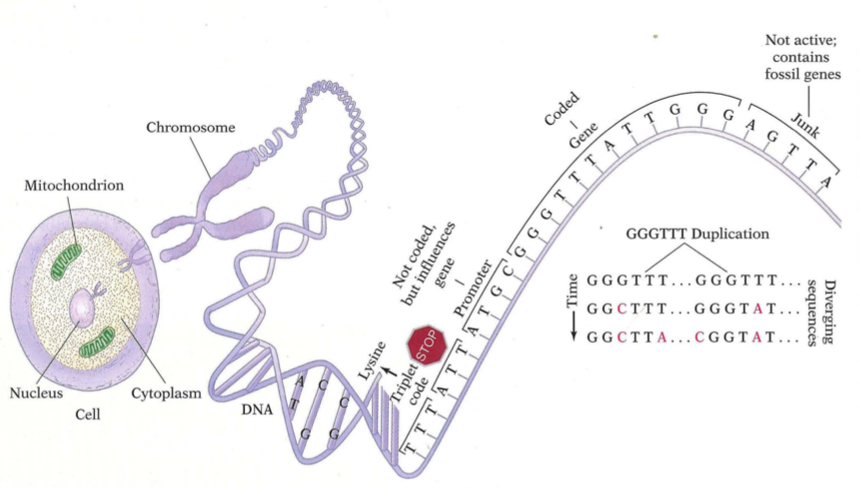
\includegraphics[width=8.0cm]{fig/chrom.png}
			\caption{ }
			\label{chrom}
		\end{figure}

		\item mutace se objevuji s pravidelnosti o periode 1 milion let
		\item tim padem starsi casti systemu maji vic mutaci (vic obmen)
			\vspace{3mm}
		\item "molekularni hodiny" jsou velmi dulezite pri odhadu skokovych zmen v evoluci mozku
			\vspace{3mm}
			\vspace{3mm}
	\end{itemize}
\end{itemize}
serotonin - priklad - Barry Jacobs: 
\begin{itemize}
	\item 
	\begin{itemize}
		\item aktivita serotoninovych neuronu je tesne spjata s vybuzenim zvirete
		\item viz obrazek kocky Obr.\ref{cat} 

		\begin{figure}[ht]
			\centering
				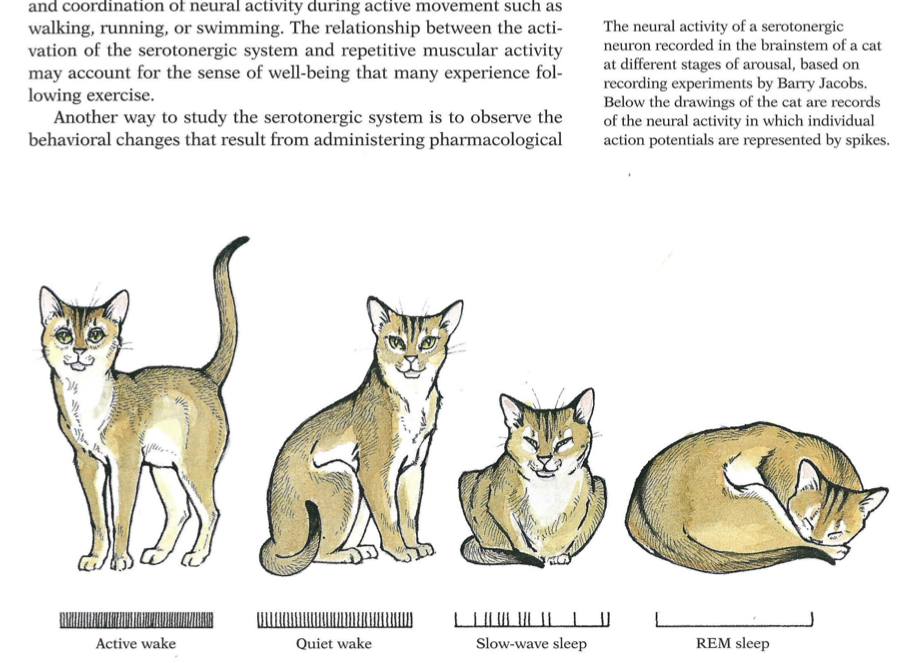
\includegraphics[width=10.0cm]{fig/cat.png}
			\caption{Souvislost aktivity serotoninovych neuronu s aktivitou zvirete}
			\label{cat}
		\end{figure}

			\vspace{3mm}
		\item aktivita serotoninovych neuronu prudce stoupne PRAVE pred svalovou aktivitou zvirete
		\item pokud je zvire hodne aktivni, jsou i serotoninove neurony aktivni, naopak v REM spanku, kdy je vetsina svalu neaktivni, jsou i tyto neurony neaktivni
			\vspace{3mm}
		\item aktivita serotogeninovych neuronu koreluje s fyzickou aktivitou zvirete, bylo to namereno i u ryb
		\item serotoninove neurony jsou tedy rizeny povelem pro svalovou aktivitu
			\vspace{3mm}
		\item serotonin funguje i jako stabilizator mozkove aktivity (napriklad ma neco spolecneho s obscesivne-kompulzivni chorobou)
			\vspace{3mm}
		\item vliv v amygdale a orbital-frontal cortexu (ktere jsou spjaty za socialni chovani)	
		\begin{itemize}
			\item ma dobry vliv na socialni chovani(pece o vzhled) a negativni na antisocialni (fighting)
			\item diky tomu serotonin moduluje chovani k ostatnim jedincum
				\vspace{3mm}
		\end{itemize}

		\item serotonin zapricinuje vetsi riskovani v prstredi
		\begin{itemize}
			\item vyssi hladina serotoninu - vetsi spokojenost, mene riskovani	
			\item mensi spokojenost - zvire vic riskuje (low serotonin monkey - predator sentinel)
				\vspace{3mm}
		\end{itemize}

		\item serotoninovy system tedy slouzi k modulaci sil spojeni mezi neurony tak, aby produkovaly stabilni chovani v rozdilnych situacich
		\item je to tak dulezite ze se tenhle system zachoval 500 milionu let
		\item snizeni serotoninu ma za nasledek zvyseni riskovani - ohrozeni a odmena - coz zvysuje adaptivitu zvirete
		\item snizeni serotoninu ale vede k mensi spokojenosti a k ruznym porucham (napriklad spanku, deprese apod)
		\item je to dulezita slozka membran nervovych bunek
		\item da se najit ve vsech slozkach potravy bohate na energii
		\item pokud ma zvire malo serotoninu, muze byt vycerpano hypersenzitivitou
			\vspace{3mm}
			\vspace{3mm}
	\end{itemize}
\end{itemize}
neocortex:
\begin{itemize}
	\item 
	\begin{itemize}
		\item nervova tkan pokryvajici vetsinu mozku
		\item serotogenicky system - u vetsiny obratlovcu stejny
		\item neocortex - nachazi se pouze u savcu
		\item Mozková kura (kura velkého mozku - neopallium - neocortex) neocortex by mel byt casti mozkove kury
		\item u cloveka nejvyznamnejsi cast mozku
		\item behem fylogenetickeho vyvoje se zvetsuje kortikalizace funknci
		\begin{itemize}
			\item do mozkove kury tedy prichazi stale vetsi mnozstvi aferentaci (dostredivych vlaken)
			\item a pod kontrolu vzruchu, ktere z kury vycahzeji se dostava cim dal vic telesnych funkci (zvire je sikovnejsi)
				\vspace{3mm}
		\end{itemize}

		\item u cloveka 200 000 cm2
		\item koreluje s velikosti tela, u nekterych velryb se zubama je prekvapive velky
			\vspace{3mm}
		\item velikost neocortexu je omezena velikosti hlavy, ta je omezena komplikacemi pri porodu, proto vrasneni
			\vspace{3mm}
			\vspace{3mm}
	\end{itemize}
\end{itemize}
Frenologie:
\begin{itemize}
	\item 
	\begin{itemize}
		\item byl obor, který predpokládal a zkoumal souvislost stavby lebky s duševními schopnostmi a charakterovými rysy. 
		\item Byl populární zejména v 19. století, do zacátku 20. století však byl zavrřen jako pseudoveda. 
		\item Nekteré predstavy o funkcní specializaci jednotlivých cástí mozku však od ní úspešně prevzala moderní neuroveda. 
		\item jednotlive casti mozku se roztahnout kdyz funguji, podle toho se meri jejich aktivita
			\vspace{3mm}
		\item experimentalni neurobiologie, nekdo se pokusil odejmout casti mozku zvirat aby potvrdil tohle, nepovedlo se
			\vspace{3mm}
	\end{itemize}
\end{itemize}
Neocortex:

Hughlings Jackson's clinical observations relate to three fundamental properties of the neocortex. 
\begin{itemize}
	\item 
		\item 
\begin{itemize}
		\begin{itemize}
			\item 1) the neocortex contains topographic maps
			\item 2) the parts of these maps which are used the most have the largest representations
			\item 3) the neocortex has a key role in the genesis of epilepsy.
				\vspace{3mm}
		\end{itemize}

		\item The cortical circuitry is highly plastic in that 
		\item it can change its functional organization in response to experience, and it is crucial for memory formation and storage.
			\vspace{3mm}
		\item price of this cortical plasticity is the risk of the wildly uncontrolled oscillations in neural activity that occur in epilepsy.
			\vspace{3mm}
		\item mnoho pokusu s motor-cortex, pri stimulaci slabymi elektrickymi pulzy se hybou svaly => slozite topograficke mapy pro ruzne svaly
		\item opice: piti z male studny (sikovnost) a piti z velke studny (pohoda)
		\begin{itemize}
			\item sikovne opice mely o hodne vetsi kortikalni reprezentaci pro prsty nez ty druhe
			\item je to videt i u lidi kteri hraji na strunny nastroj nebo u slepcu - Brailovo pismo 
			\item lepsi a presnejsi kontrola = vetsi reprezentace v kortexu
				\vspace{3mm}
				\vspace{3mm}
				\vspace{3mm}
				\vspace{3mm}
		\end{itemize}
	\end{itemize}
\end{itemize}
hippocampus:
\begin{itemize}
	\item 
	\begin{itemize}
		\item oblibeny pro studie pameti
			\vspace{3mm}
			\vspace{3mm}
			\vspace{3mm}
	\end{itemize}
\end{itemize}
Striatum (též corpus striatum, lat. žíhané jádro) 
\begin{itemize}
	\item 
	\begin{itemize}
		\item je hluboká oblast šedé hmoty uvnitr hemisfér koncového mozku. 
		\item Je to zrejme rozsahem nejvýznamnejší soucást tzv. bazálních ganglií
			\vspace{3mm}
		\item Do striata smerují dráhy nejen z mozkové kury, ale i z nekterých subkortikálních (podkorových) center, thalamu a z mozkového kmene. 
		\item Z bazálních ganglií je to zrejme vubec nejvýznamnejší príjemce signálu z jiných cástí mozku. 
		\item Naopak z striata smerují dráhy do globus pallidus (nepocítáme-li ho do striata), ale i napr. do substantia nigra.

Oblast globus pallidus (nekdy považovaná za samostatné jádro šedé hmoty stojící mimo striatum) hraje duležitou roli v ovládání pohybu, jelikož z neho smerují dráhy do retikulárních formací v mozkovém kmeni a (pres thalamus) i do pohybových center v mozkové kure. 
	\end{itemize}
\end{itemize}

\end{document}
